\documentclass{scrreprt}
\usepackage{graphicx}
\usepackage{listings}
\usepackage{underscore}
\usepackage[bookmarks=true]{hyperref}
\usepackage[utf8]{inputenc}
\usepackage[english]{babel}
\usepackage{subfigure}
\usepackage{hyperref}
\usepackage[table,xcdraw]{xcolor}
\setlength{\footskip}{140pt}
\graphicspath{ {images/} } 
\hypersetup{
    bookmarks=false,    % show bookmarks bar?
    pdftitle={Design and Project Management Update},    % title
    pdfauthor={Matthew Berger},                     % author
    pdfsubject={TeX and LaTeX},                        % subject of the document
    pdfkeywords={TeX, LaTeX, graphics, images}, % list of keywords
    colorlinks=true,       % false: boxed links; true: colored links
    linkcolor=blue,       % color of internal links
    citecolor=black,       % color of links to bibliography
    filecolor=black,        % color of file links
    urlcolor=purple,        % color of external links
    linktoc=page            % only page is linked
}%
\def\myversion{1.0 }
\date{}
%\title
\usepackage{xcolor,colortbl}
\newcommand{\mc}[2]{\multicolumn{#1}{c}{#2}}
\definecolor{LightGray}{gray}{0.95}
\definecolor{Gray}{gray}{0.85}
\definecolor{LightCyan}{rgb}{0.88,1,1}

\newcolumntype{a}{>{\columncolor{Gray}}p{0.3\linewidth}}
\newcolumntype{b}{>{\columncolor{white}}p{0.7\linewidth}}
\newcolumntype{d}{>{\columncolor{LightGray}}p{0.3\linewidth}}
\newcolumntype{e}{>{\columncolor{white}}p{0.6\linewidth}}
\newcolumntype{f}{>{\columncolor{LightGray}}p{0.2\linewidth}}
\newcolumntype{g}{>{\columncolor{Gray}}p{0.2\linewidth}}
\newcolumntype{h}{>{\columncolor{white}}p{0.8\linewidth}}

\begin{document}

\begin{flushright}
    \rule{16cm}{5pt}\vskip1cm
    \begin{bfseries}
        \Huge{PROJECT MANAGEMENT SPECIFICATIONS}\\
        \vspace{1.6cm}
        for\\
        \vspace{1.6cm}
        $NAVATAR$\\
        \vspace{1.6cm}
        \LARGE{Version \myversion approved}\\
        \vspace{1.6cm}
        Prepared by Matthew Berger, Liam Gomez, and Connor Parkinson\\ 
        \vspace{1.6cm}
        Advised by Professor Eelke of the\\UNR CSE Department\\
        \vspace{1.6cm}
        \today\\
    \end{bfseries}
\end{flushright}

\tableofcontents

\chapter{Abstract}
Navatar is an indoor navigation system for visually impaired students. Unlike existing systems that rely on expensive equipment, Navatar only requires an Android smartphone. The phone’s GPS, accelerometer, and compass are used to approximate a user’s location and movements and the phone’s speaker is used to provide auditory directions to rooms within a building. Buildings on University campuses often have the GIS maps and the design required for Navatar’s accelerometer and compass based localization, which is why students are the intended audience for the project. With the application’s open source status and modular design, crowdsourcing efforts can be used to integrate maps for buildings on any campus. The application is still under development and Team 6 is working on project management and scheduling for the implementation of a variety of new features alongside other open source contributors.


\chapter{Project Updates and Changes}
Team 6 has been working on cleaning up the existing code base to better facilitate the implementation of the planned features while also debugging issues encountered with the existing code. The team has recently added additional priority to fixing bugs with the existing maps and map creation functionality as their advisor, Eelke Folmer, informed them a university has expressed interest in the development of Navatar. Efforts are also being made to automate setup of the development environment to allow other open source contributors to easily assist with improving Navatar.
It became evident after the design and prototype stage that some of the team's ideas were better in theory than in implementation. One such example was the gesture-detection as a form of interaction with the application. Gestures that are context-aware lead to the same application interactions eliciting separate and highly distinct behaviors that may lead to unexpected results for the user. The context of the application may be difficult to discern for a blind user. In this sense, gesture-detection should be superseded and brought to obsolescence by voice commands. We changed our design to use Google voice to implement the actual voice recognition and voice commands. Simply speaking to the application through a microphone on a headset or set of ear-buds will allow for more accurate control and potentially limitless interactions with the app that gestures simply would not allow for. There are only a limited number of gestures, and the overlap with existing accessibility applications would make the usability ineffective. Voice commands are the chosen options here. After designing, prototyping, and testing the GPS features we found that reliably detecting a user’s location indoors was difficult. It was determined that the real use-case for autolocation would be when a user enters a building, which allows for the best location accuracy using GPS. The subsequent use cases including the user leaving the building or navigating between rooms inside the building are made possible using an Android feature that allows for getting the last known location of the smartphone.The autolocation functionality is done using Geo-Fencing currently, and can be improved by using additional location data sources such as WiFi or cellular towers. As for navigation history, it is a nearly complete and functional feature barring the additional planned functionalities of allowing users to reverse the previously navigated route and collecting data on which routes are completable. Additional focus for improving the feature is allowing users to navigate the selections with easily spoken voice commands. Overall there is much to work on and many features to develop with the overarching task of refactoring the codebase to improve the quality of the existing code.

\chapter{Project Deliverables}
This team’s primary focus is implementing new features that enhance the accuracy and usability of the existing application. Each team member will be responsible for the development and implementation of their respective component outlined below.

\section{Route History - Liam Gomez}
This component is responsible for logging and storing a user’s previously taken routes. Storing the previous taken routes allows for a route repeat feature to be implemented, where a user has the option to view their route history and start a new navigation from that history. Storing route history also allows for a user to a reverse a given navigation after reaching their destination.

\subsection{User Stories}
\begin{enumerate}
	\item As a user, after opening Navatar, I should be given an option that takes me to the route history page so I can view my route history.
	\item As a user, on the route history page, I should be able to select a route from my history so I can repeat that navigation.
	\item As a user, after successfully completing a navigation, I should be prompted if I would like to reverse that route so I can navigate back to my origin.
	\item As a user, on the route history page, I would like to avoid having failed or incomplete navigations saved to my history so I can avoid repeating them.
	\item As a researcher, I should have access to the route history logs in a parsable format for analytical purposes.
\end{enumerate}

\pagebreak

\section{Geofencing - Connor Parkinson}
This component is responsible for the automatic selection of the campus and building based on the user’s current location. This component will use a combination of the smartphones GPS, cellular, and Wi-Fi to provide locational data. This locational data will then be compared with the known geographical boundaries of available campuses and buildings.

\subsection{User Stories}
\begin{enumerate}
	\item As a user, I want Geofencing so that I don't have to select the campus I am on.
	\item As a user, I want Geofencing functionalities to be active when I open the app.
	\item As a user, I want to revert to existing campus and or building selection if Geofencing fails (is not accurate enough or times out).
	\item As a user, I want Geofencing so that I don't have to select the building I want to navigate within.
	\item As a user, I want Geofencing to select at least the campus even when accuracy is not high enough to select the building.
\end{enumerate}

\pagebreak

\section{Gesture-Based Controls - Matthew Berger}
This component is responsible for providing an additional input method to the user that is outside the existing Google Talkback integration. For a user with visual impairments navigating content heavy menus and input fields can be quite tedious. To improve this, a gesture based input system will be implemented and integrated with the existing user interface. Gesture based input will allow the user to make gestures on their devices screen that control the applications behavior.

\subsection{User Stories}
\begin{enumerate}
	\item As a user, I want to be able to control the application without having to speak in noisy environments.
	\item As a user, I want gestures to be consistent, intuitive, and reliable.
	\item As a user, I want to be able to long press to add a landmark.
	\item As a user, I want gestures to be available for the entire screen, not a subsection.
	\item As a user, I want to be able to swipe to confirm or reject application prompts.
\end{enumerate}

\chapter{Project Assignments and Schedule}
Our group is using the ZenHub chrome extension in combination with Github's issue tracker for project management. Using this tool, it has been very easy to assign work items to the members of group as well as manage collections of similar features and categorize desired and existing features. As of now, all of the major work items listed under the 'Spring 2017 Desired Features' epic on the Github repository's issue tracker can be feasibly achieved by the end of the semester on May 5th. All other features listed on the tracker are there for future reference but are not vital to the success of the project as it stands this semester. Navatar is a free and open-source software project, therefore it is important to make a note of any and all issues as they come up. We have specifically selected the most important issues to be included in our epic for the semester.

\href{https://github.com/matthewjberger/navatar/}{Click here to view the Navatar repository on Github.}

\pagebreak

\section{The Zenhub Scrum Board}

With the ZenHub chrome extension installed, the Github issue tracker gets an extended set of features more suited to scrum project management. One such feature is a scrum board that's directly linked to Github issues on your github repositories. In our case, the issues we've created for Navatar can be categorized and managed on the scrum board through the 'board' tab that's added along with ZenHub.

\href{https://github.com/matthewjberger/navatar/issues\#boards?repos=80390803}{Click here to view the full scrum board on Github (if you have the ZenHub chrome extension installed).}

\begin{figure}[ht!]
     \begin{center}
%
        \subfigure[The Full Scrum Board]{%
            \label{fig:first}
            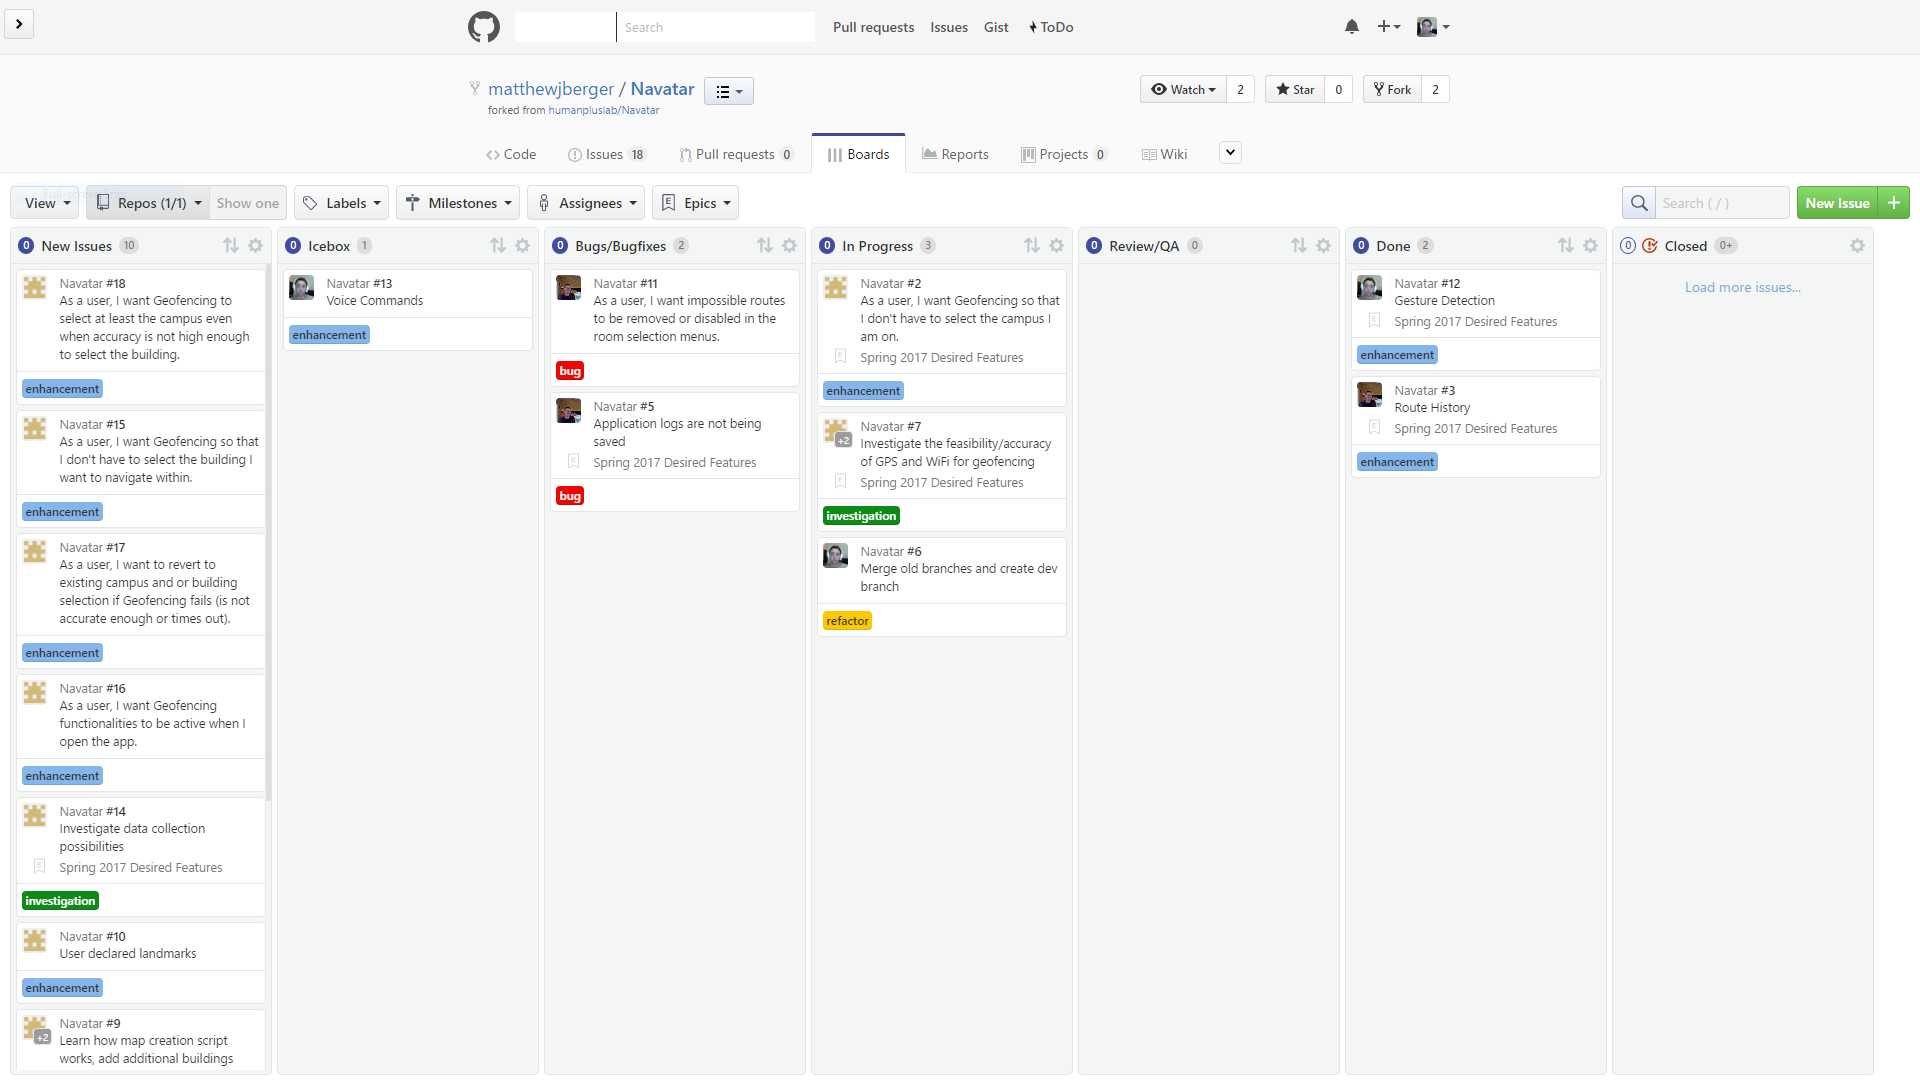
\includegraphics[width=\textwidth,height=\textheight,keepaspectratio]{scrumboard.png}
        }\\%
        \subfigure[A Close-Up of the Scrum Board]{%
            \label{fig:second}
            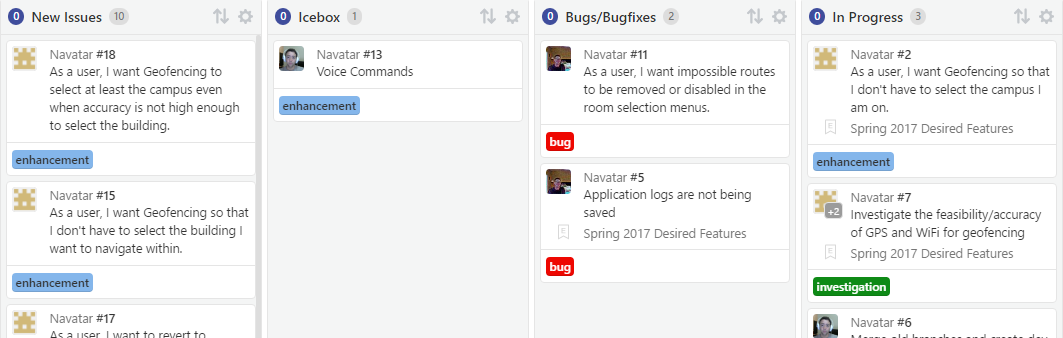
\includegraphics[width=\textwidth,height=\textheight,keepaspectratio]{scrumboardcloseup.png}
        }\\%
    \end{center}
    \caption{%
        Scrum Board Screenshots
     }%
   \label{fig:subfigures}
\end{figure}

\pagebreak

\section{Github Issue Tracking with the Zenhub Extension}

\subsection{Epic Issues}

One feature that's added with the extension is Epic issue management. Epic issues are collections of issues to be prioritized and completed, and any issues created after an epic is made have the option to be assigned to an existing epic.

\href{https://github.com/matthewjberger/navatar/issues}{Click here to view the full issue tracker on Github.}

\begin{center}
\begin{figure}[ht!]
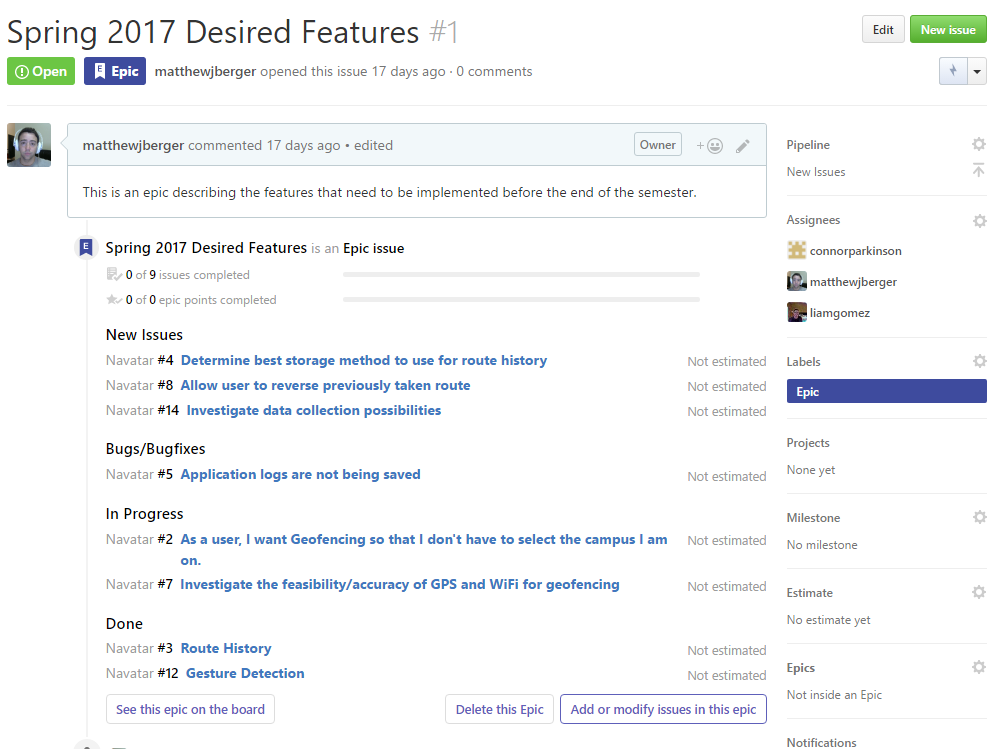
\includegraphics[width=\textwidth,height=\textheight,keepaspectratio]{epic.png}
\caption{An epic issue.}
\end{figure}
\end{center}

\pagebreak

\subsection{Issue Categorization}

Issues on Github can be labeled and assigned authors in order to make finding and identifying issues more accessible. With Github's issue tracker, all of the issues listed are searchable by tag, name, author, and date through Github's built-in search capabilities. Each issue contains a conversation about the issue, and can reference other issues, commits, repositories, etc as well be resolved or closed categorically by a collaborator on the repo. These changes are all automatically reflected on the scrum board via the ZenHub chrome extension.

\begin{figure}[ht!]
     \begin{center}
%
        \subfigure[Labeled issues on the board.]{%
            \label{fig:first}
            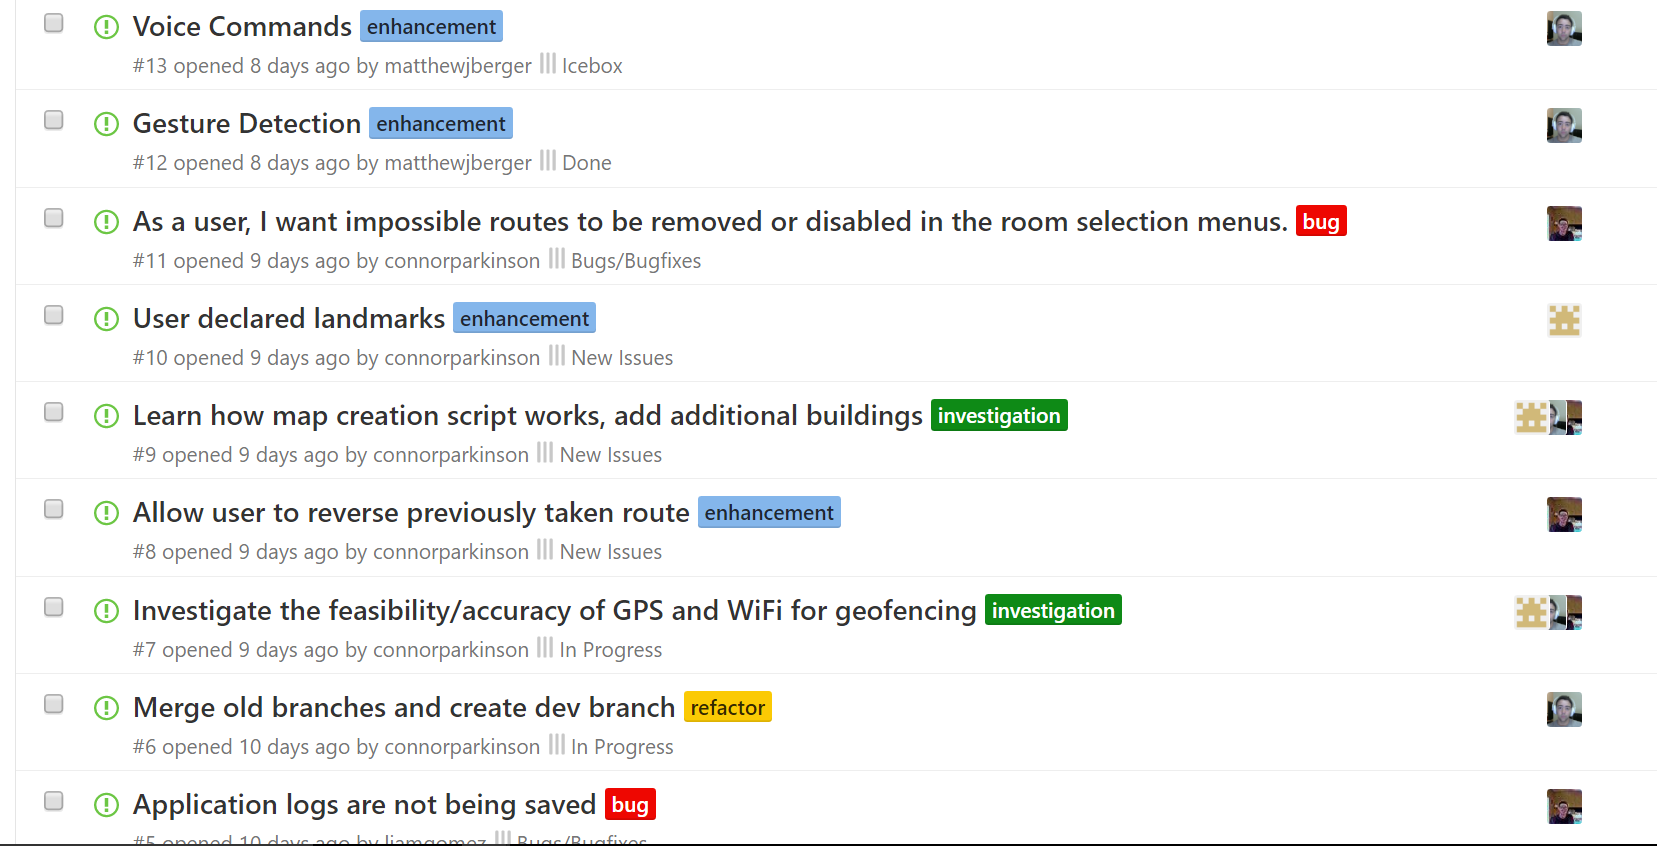
\includegraphics[width=\textwidth,height=0.3\textheight,keepaspectratio]{issues.png}
        }\\%
        \subfigure[A Navatar issue discussion on Github.]{%
            \label{fig:second}
            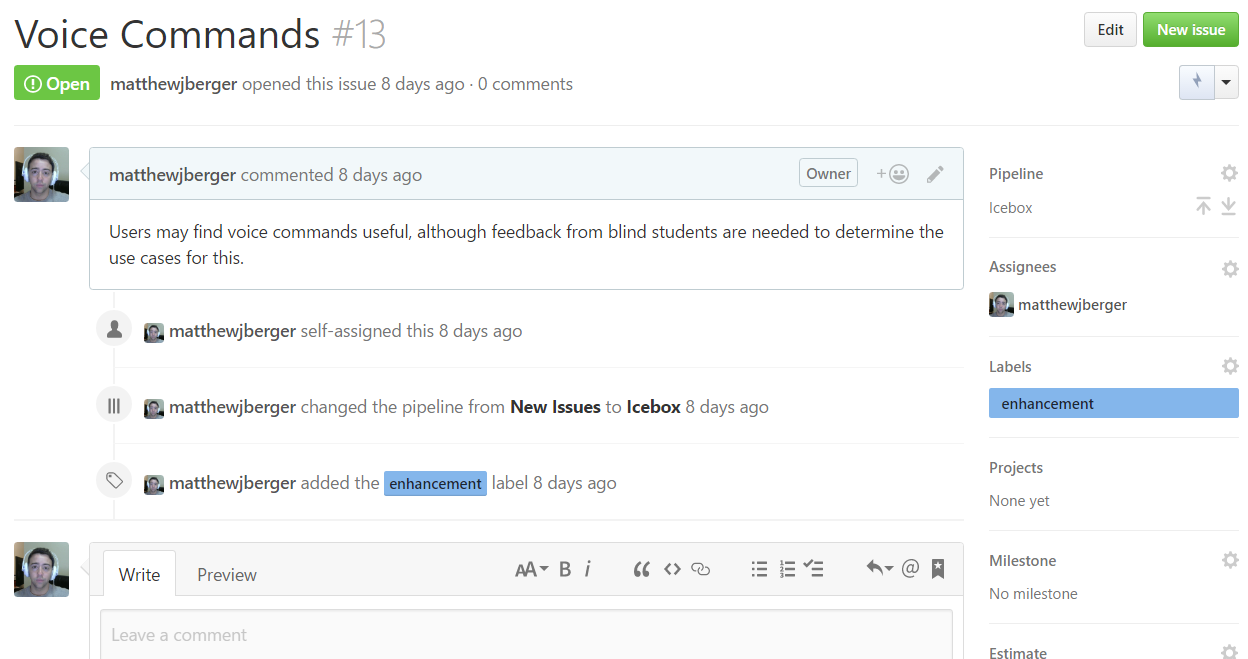
\includegraphics[width=\textwidth,height=0.3\textheight,keepaspectratio]{openissue.png}
        }\\%
    \end{center}
    \caption{%
        Scrum Board Screenshots
     }%
   \label{fig:subfigures}
\end{figure}

\pagebreak

\section{Branching Model}

A successful git branching model is vital for organized but quick development of a project. In our project, we plan to follow the github branching model detailed below.

\href{http://nvie.com/posts/a-successful-git-branching-model/}{Click here to view the article discussing this branching model.}

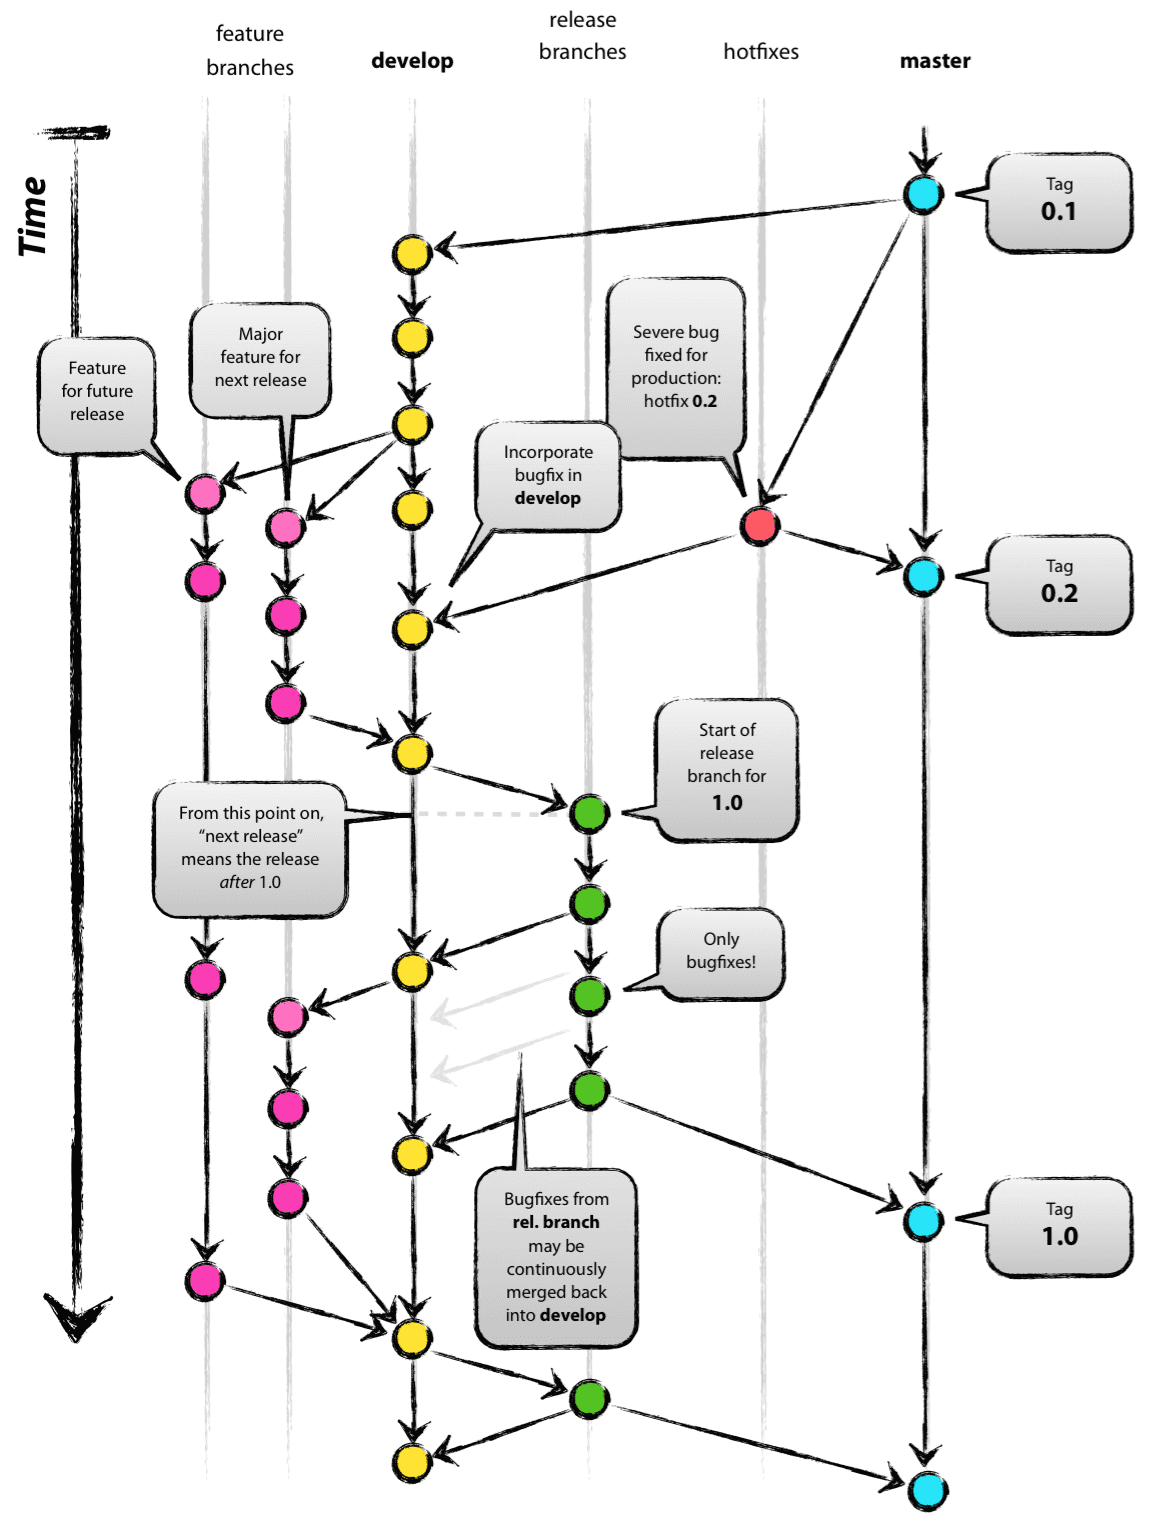
\includegraphics[width=\textwidth,height=0.8\textheight,keepaspectratio]{branchingmodel.png}

\chapter{Project Monitoring and Risk}

Following the updates to the requirements and design of the planned features, the team developed a schedule and timeline to ensure project success. The team delegated subsystems, responsibilities, and workload by having each team member volunteer for pre-established subsections and responsibilities based on their experience and interests. Project tasks were outlined on the scrum board with corresponding time estimates and the team developed the schedule with both realistic and stretch goals for what is planned to be accomplished. Weekly meetings have been established which allows for all team members to hold each other accountable for their assigned tasks and for the team to reallocate time for tasks which could be deemed more complex than originally anticipated. A Gantt chart was considered for outlining each scheduled task and dependencies, but the team deemed it unnecessary due to the independent design of each planned feature.

\section{Risk Management Strategies}
\begin{enumerate}
	\item[] \textbf{Sudden Increase in Requirements or Development time}
	\item Mitigating the risk of sudden requirement or time increases has been mitigated by thoroughly establishing the requirements and design with a corresponding schedule that allows for flexible time allocation.
	\item[] \textbf{Productivity Issues}
	\item By having a realistic schedule and frequent team meetings, the team members are held accountable for the progress expected to be achieved at every step of the development process.

	\item[] \textbf{Scheduling Issues}
	\item Establishing frequent team meetings is possible by having all team members commit early in the development process to certain times and dates with sufficient time to prioritize and plan.

	\item[] \textbf{Bugs with the Existing Codebase}
	\item The team understands that issues can arise when working with existing code which is why the planned features have been designed to be as modular as possible to avoid conflicts with existing code. The team has also allotted time for debugging essential functionalities.
	
\pagebreak

	\item[] \textbf{Development Environment Consistency}
	\item Developing an application for Android involves a multitude of version specific dependencies which can be difficult to maintain and resolve conflicts between. The team is using Vagrant to configure a standard which is being used by all team members and will be suggested for all other open source contributors.

	\item[] \textbf{Unit Test Coverage}
	\item The application has a lot of existing code, and such code may or may not be guaranteed to work. To ameliorate this and provide a safe way forward, we intend to write tests for portions of the code that we touch in order to preserve the functionality in place and assure that new functionality is robust and well-integrated.
	
	\item[] \textbf{Scope Creep}
	\item There are many modular features planned, but approaching too many at once can lead to a large increase in the amount of time per task and ultimately prevent the app from seeing completion by the end of the semester. To prevent this, we are planning out the project carefully and assigning specific, isolated, and modular features to members of the group and allowing an ample amount of time to complete and integrate them. This will help to prevent scope creep, and assure functionality is added to the software by the deadline.
	
	\item[] \textbf{Development Conflicts}
	\item To properly manage the project on github and ensure each developer can work on the project properly and without breaking the codebase, we will follow the git branching model listed in this document and be deliberate in our usage of branches and commits. All commits will contain a full and accurate commit message. Additionally, continous integration will be used to run unit tests on each commit so at a glance it will be known whether or not a prior commit broke the build and we can address the issue with expedience.
	
	\item[] \textbf{Team Coordination}
	\item Without proper communication, the team will not be able to coordinate their activities and develop properly. The simple solution we have come up with is to use sms, google hangouts, and shared google documents to properly interact without each other for our project necessities.
	
	\pagebreak
	
	\item[] \textbf{Team Motivation}
	\item To prevent the team from becoming overwhelmed by deadlines and features, milestones will be set and will contain small goals that comprise the larger issues. This will assure constant progress and will keep the team motivated to continue working on the project. Additionally, to motivate others to work on the project we will make the repository and codebase more friendly by adding contribution guidelines and explaining how to build the source code with the development environment provided by our vagrant box. Having other people open pull requests and submit issues will help develop the project and boost team morale.
\end{enumerate}

\chapter{Team Contributions}
	\section{Matthew Berger}
		\begin{itemize}
			\item Created LaTeX document
			\item Setup source and development environment controls
			\item Completed project assignments and schedule
			\item Created gesture subsystem user stories
			\item Completed five of the ten risk management strategies
		\end{itemize}
	\section{Connor Parkinson}
		\begin{itemize}
			\item Completed the abstract
			\item Outlined the project design and requirement updates
			\item Established the project monitoring plan
			\item Completed five of the ten risk management strategies
		\end{itemize}
	\section{Liam Gomez}
		\begin{itemize}
			\item Outlined the project deliverables
			\item Organized user stories on the team’s ZenBoard
			\item Compiled the references.
		\end{itemize}
	\section{All Team Members}
		\begin{itemize}
			\item Peer review, editing, and formalization of this document and the knowledge contained herein.
		\end{itemize}
\end{document}

